\chapter{Structure, Guidelines, New Folder Setup}

\section{Directory Structure}

We briefly describe the directory structure of \Dumux in terms 
of subdirectories, source files, and tests. For more details, 
the Doxygen documentation should be considered. 
\Dumux comes in form of a DUNE module \texttt{dumux}. 
It has a similar structure as other DUNE modules like \texttt{dune-grid}. 
The following subdirectories are within the module's root directory, 
from now on assumed to be \texttt{/}: 
\begin{itemize} 
\item \texttt{CMake}: the configuration options 
for building \Dumux using CMake. See the file \texttt{INSTALL.cmake} in 
the root directory of \texttt{dumux} for details. Of course, 
it is also possible to use the DUNE buildsystem just like for the other 
DUNE modules.
\item \texttt{doc}: contains the Doxygen documentation in \texttt{doxygen}, 
this handbook in \texttt{handbook}, and the \Dumux logo in various formats in 
\texttt{logo}. The html documentation produced by Doxygen can be accessed as usual, 
namely, by opening \texttt{doc/doxygen/html/index.html} with a web browser. 
\item \texttt{dumux}: the \Dumux source files. See Section \ref{sec:dumux} for details. 
\item \texttt{test}: tests for each numerical model and the property system. 
See Section \ref{sec:test} for details. 
\item \texttt{tutorial}: contains the tutorials described in Chapter \ref{chp:tutorial}. 
\end{itemize}



\subsection{The directory \texttt{dumux}}\label{sec:dumux}

The directory \texttt{dumux} contains the \Dumux source files. It consists of the following subdirectories (see Figure \ref{fig:dumux-structure}): 

\begin{itemize} 

\item \texttt{boxmodels}:
the general fully implicit box method is contained in the subdirectory 
\texttt{common}, while each of the other subdirectories contains 
a derived specific numerical model. The subdirectory \texttt{common} also contains the file \texttt{boxfvelementgeometry.hh} employed by the box method to extract the dual mesh geometry information out of the primal one. The files \texttt{pdelabboxassembler.hh} and \texttt{pdelabboxlocaloperator.hh} allow the use of the DUNE module \texttt{dune-pdelab}. 

\item \texttt{common}:
general stuff like the property system and the time management for the 
fully coupled as well as the decoupled models, the interface for the Pardiso direct solver library \cite{Pardiso}, and the \texttt{start.hh} file that includes the common routine for starting a model called in the main function. 

\item \texttt{decoupled}:
 numerical models to solve the pressure equation as part of the fractional flow formulation. The specific models are contained 
 in corresponding subdirectories. In each model folder are subdirectories for the implicit pressure equation sorted by the employed discretization method, and for the explicit transport equation. The general decoupled formulation for the implicit pressure explicit transport formulation can be found in the subdirectory \texttt{common}.

% \item \texttt{fractionalflow}:
% the (non-compositional) fractional flow model, which utilizes the IMPES method 
% contained in the subdirectory \texttt{impes}.

% \item \texttt{functions}:
% the Crouzeix--Raviart function implemented in the style of \texttt{dune-disc}'s P1 function. 

% \item \texttt{fvgeometry}:
% employed by the box method to extract the dual mesh geometry information out of the 
% primal one. 

\item \texttt{io}: additional in-/output possibilities like restart files 
and a VTKWriter extension. 

\item \texttt{material}: everything related to material parameters and 
constitutive equations. The properties of a pure chemical substance (e.g. water) or pseudo substance (e.g. air) can be found in the subdirectory \texttt{components} with the base class \texttt{components/component.hh}. The fluidsytem in the folder \texttt{fluidsystems} collects the information from the respective component and binary coefficients files, and contains the fluid characteristics of phases (e.g. viscosity, density, enthalpy, diffusion coefficients) for compositional or non-compositional multi-phase flow. 

The base class for all spatially dependend variables -- like permeability and porosity  -- 
can be found in \texttt{spatialparameters}. The base class in \texttt{boxspatialparameters.hh} 
also provides spatial averaging routines. All other spatial properties are specified in the specific
 files of the respective models. Furthermore, the constitutive relations -- e.g. $p_c(S_w) $ -- are in \texttt{fluidmatrixinteractions}, 
while the necessary binary coefficients like the Henry coefficient or binary diffusion coefficients are definded in
 \texttt{binarycoefficients}.


\item \texttt{nonlinear}: Newton's method.


% \item \texttt{operators}: based on \texttt{dune-disc}, assembly operators for Crouzeix--Raviart 
% elements and mimetic finite differences. 
% 
% 
% \item \texttt{pardiso}: interface to the Pardiso direct solver library, \cite{Pardiso}. 
% 
% 
% \item \texttt{shapefunctions}:  Crouzeix--Raviart element shape functions. 
% 
% 
% \item \texttt{timedisc}: time discretization for the decoupled models. 
% 
% 
% \item \texttt{transport}: numerical models to solve the pressure equation 
% as part of the fractional flow formulation analogous to the \texttt{diffusion} 
% directory. Moreover, the compositional decoupled models are included here. 


\end{itemize}



\subsection{The directory \texttt{test}}\label{sec:test}


The directory \texttt{test} contains a test for each numerical model and for 
the property system. The tests for the property system and the pardiso solver can be found in \texttt{common}. 
The subfolder \texttt{boxmodels} contains tests for the fully 
coupled models (\texttt{1p},  \texttt{1p2c},  \texttt{2p},  \texttt{2p2c},  
\texttt{2p2cni},  \texttt{2pni},  and \texttt{richards}), while the subdirectory \texttt{decoupled} corresponds to the decoupled models. 
Each subdirectory contains one or more program files \texttt{test\_*.cc}, where \texttt{*} usually is the 
name of the folder. Moreover, the problem definitions can be found 
in the \texttt{*problem.hh} files and the definition of the spatially dependend parameters in \texttt{*spatialparameters.hh}. Simply executing the tests should either run the 
full test or give a list of required command line arguments. After test execution, 
VTK output files should have been generated. 
For more detailed descriptions of the tests, the problem definitions and their corresponding 
Doxygen documentation should be considered. 

\begin{landscape}
\begin{figure}[hbt]
  \centering 
  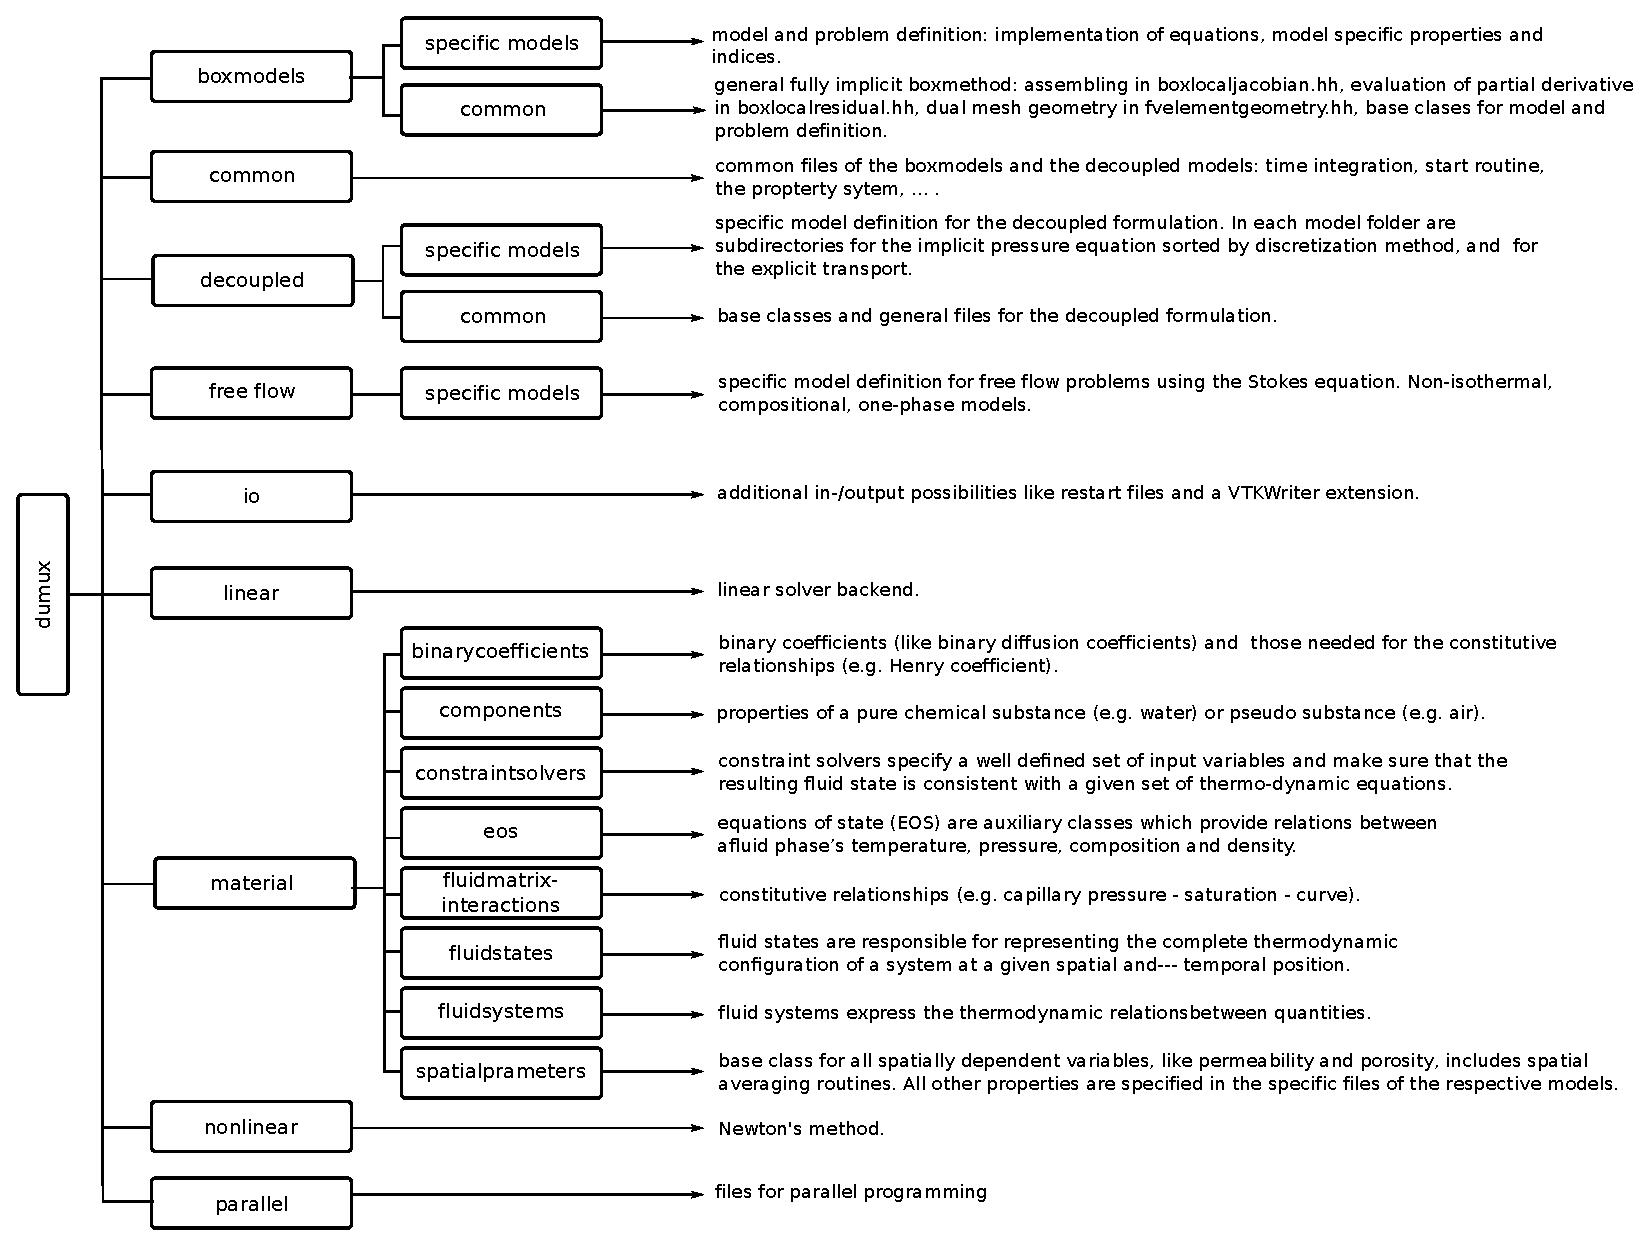
\includegraphics[width=\linewidth, keepaspectratio]{EPS/dumux_strucutre_flowchart_horizontal_explained.eps}
  \caption{
    \label{fig:dumux-structure}
    Structure of the directory \texttt{dumux} containing the \Dumux source files.
  }
\end{figure}
\end{landscape}

\section{Guidelines} 
\label{guidelines}

This section adaptes the DUNE coding guidelines found at \cite{DUNE-HP}. 
These guidelines also should be followed by every \Dumux developer and user. \\
In order to keep the code maintainable we have decided upon a set of coding rules. 
Some of them may seem like splitting hairs to you, but they do make it much easier 
for everybody to work on code that hasn't been written by oneself.

\begin{itemize}
\item Naming: 
\begin{itemize}
\item Comments: they are helpful! Please document freely what each part of your code does. 
\item all comments / documentation is in english
\item Variables: Names for variables should only consist of letters and digits. The first letter should be a lower case one. If your variable names consists of several words, then the first letter of each new word should be capital. As we decided on the only exception are the begin and end methods.
\item variables should be named as self-explaining as possible: especially abbreviations should be avoided (saturation in stead of S)
\item Private Data Variables: Names of private data variables end with an underscore and are the only variables that contain udnerscores. 
\item Typenames: For typenames, the same rules as for variables apply. The only difference is that the first letter should be a capital one.
\item Macros: The use of preprocessor macros is strongly discouraged. If you have to use them for whatever reason, please use capital letters only.
\item The Exlusive-Access Macro: Every header file traditionally begins with the definition of a preprocessor constant that is used to make sure that each header file is only included once. If your header file is called 'myheaderfile.hh', this constant should be DUNE\_MYHEADERFILE\_HH.
\item Files: Filenames should consist of lower case letters exclusively. Header files get the suffix .hh, implementation files the suffix .cc
\end{itemize}
\item Documentation:
      Dune, as any software project of similar complexity, will stand and fall with the quality of its documentation.
Therefore it is of paramount importance that you document well everything you do! We use the doxygen system to extract easily-readable documentation from the source code. Please use its syntax everywhere. In particular, please comment \textbf{all}
\begin{itemize}
\item Method Parameters (in / out)
\item Template Parameters
\item Return Values 
\item Exceptions thrown by a method
 \end{itemize}
     Since we all know that writing documentation is not well-liked and is frequently defered to some vague 
'next week', we herewith proclaim the Doc-Me Dogma . It goes like this: Whatever you do, and in whatever hurry you 
happen to be, please document everything at least with a {\verb /** $\backslash$todo Please doc me! */}. That way at least the absence 
of documentation is documented, and it is easier to get rid of it systematically.
\item Exceptions:
      The use of exceptions for error handling is encouraged. Until further notice, all exceptions thrown are DuneEx.
\item Debugging Code:
      Global debugging code is switched off by setting the symbol NDEBUG. In particular, all asserts are 
automatically removed. Use those asserts freely!
\end{itemize}

\section{Setup of a New Folder}

In this section setting up a new folder is described. In fact it is very easy to create a new folder, but getting \Dumux to know the new folder takes some steps which will be explained in mroe detail below:

\begin{itemize}
 \item create new folder with content
 \item adapt \verb+Makefile.am+
 \item insert new folder in \verb+Makefile.am+ of the directory above
 \item adapt \verb+configure.ac+ in the \verb+$DUMUX_ROOT+ (the directory you checked out, probably dune-mux)
 \item newly compile \Dumux
\end{itemize}

\noindent In more detail:

\textbf{First} of all, the new folder including all relevant files needs to be created (see Section \ref{tutorial-coupled} and \ref{tutorial-decoupled} for desccription of a problem). 

\textbf{Second}, a new \verb+Makefile.am+ for the new Folder needs to be created. It is good practize to simply copy an existing file. For example the file \verb+$DUMUX_ROOT/test/2p/Makefile.am+ looks as follows:
\begin{verbatim}
bin_PROGRAMS = test_2p

test_2p_SOURCES = test_2p.cc
test_2p_CXXFLAGS = $(MPI_CPPFLAGS) 
test_2p_LDADD = $(MPI_LDFLAGS) 

include $(top_srcdir)/am/global-rules
\end{verbatim}

All occurences of \verb+test_2p+ need to be replaced by the name of the new project, e.g. \verb+New_Project+. At least if the name of the source file as well as the name of the new project are \verb+New_Project+.

\textbf{Third}: In the directory above your new Project there is also a \verb+Makefile.am+ . In this file the subdirectories are listed. As you introduced a new subdirectory, it needs to be included here. In this case the name of the new Folder is \verb+New_Project+ . Don't forget the trailing backslash.

\begin{verbatim}
 SUBDIRS = . \
	  1p \
	  1p2c \
	  2p \
	  2p2c \
	  2p2cni \
	  2pni \
	New_Project \
...
\end{verbatim}

\textbf{Fourth}: In \verb+$DUMUX_ROOT+ there is a file \verb+configure.ac+. In this file, the respective Makefiles are listed. After a line reading

 \verb+AC_CONFIG_FILES([Makefile+ 

 \noindent a line, declaring a new Makefile, needs to be included. The Makefile itself will be generated automatically. For keeping track of the included files, inserting in alphabetical order is good practice. The new line could read: \verb+test/New_Project/Makefile+ 

\textbf{Fifth}: Compile \Dumux as described in Section \ref{install}.






